% all-in-one cheatsheet layout (Michael Franzen, 2013)
\documentclass[a4paper]{article}

% geometry settings
\usepackage[top=2cm, bottom=2.5cm, left=2cm, right=2cm]{geometry}

% font settings
%\usepackage[light,math]{kurier}
\usepackage[T1]{fontenc}
\usepackage[utf8]{inputenc}
\usepackage{marvosym}
\usepackage{amssymb}
\usepackage{amsfonts}
\usepackage{amsmath}
\usepackage{amsthm}

% colors
\usepackage{xcolor}
\definecolor{lightgray}{gray}{0.8}

% formatting
\usepackage{paralist}
\usepackage{multicol}
\usepackage{tabularx}
\usepackage{Tabbing}
\usepackage{booktabs}
\usepackage{fancyhdr}
\usepackage{url}
\usepackage{mdframed}
\pagestyle{fancy}

% math
\usepackage{array}
\usepackage{eqnarray}

% figures
\usepackage{wrapfig}
\usepackage{subfig}

% figure modules
\usepackage{graphicx}
\usepackage{tikz}
\usetikzlibrary{positioning,calc}
\usepackage{algorithm2e}
\usepackage{verbatim}

% TOC & Glossary
\usepackage{sectsty}
\usepackage[nottoc,notlof,notlot]{tocbibind}
\usepackage[titles,subfigure]{tocloft}

% commands
\usepackage{xargs}
\usepackage{ifthen}

% head line
\fancyhf{}
\chead{Graph Theory - Sheet 1 - \today\\J. Batzill (1698622), M. Franzen (1696933), J. Labeit (1656460)}
\renewcommand{\headrulewidth}{0.4pt} %obere Trennlinie

\newcommand{\sheetnumber}{1}

% (problem number)
\surroundwithmdframed[
    hidealllines=true,
    backgroundcolor=gray!10,
    skipbelow=\baselineskip,
    skipabove=\baselineskip
]{mylemma}

\surroundwithmdframed[
	linecolor=white,
	skipbelow=\baselineskip,
	skipabove=\baselineskip
]{mytheorem}

\begin{document}
	
	\newtheorem{mytheorem}{Theorem}[section]
	\newtheorem{mylemma}{Lemma}[mytheorem]	

	\newenvironmentx*{solution}[1]{\section*{Problem #1}\addtocounter{section}{1}\setcounter{mylemma}{0}\setcounter{mytheorem}{0}}{}
	\newenvironmentx*{theorem}[1]{\begin{mytheorem}#1\begin{proof}}{\end{proof}\end{mytheorem}}
	\newenvironmentx*{lemma}[1]{\begin{mylemma}#1\begin{proof}}{\end{proof}\end{mylemma}}


	\begin{solution}{1}
		\begin{theorem}{Any tree $T$ has at least $\Delta(T)$ leaves.}

			\begin{lemma}{In a tree $T=(V, E)$, every path that cannot be appended ends with a leaf.}
				Let $v \in V$ be the last vertex of such a path. \\
				Assume $v$ is not a leaf then $d(v) > 1$, because $v$ has an incoming edge and is no leaf.
				According to the degree of $v$ and the fact there is no cycle in the path, we are able to increase the length of the path
				by inserting the non-used edge of $v$, a contradiction to the path's property.
				Therefore, $v$ has no more edges left which are not already included in the path. In other words, $v$ is a leaf.
			\end{lemma}	
			\begin {lemma}{In a tree, any two vertices in a graph are joined by a unique path.}
				For any two vertices within a tree, there is exactly one path joining them. Otherwise, there was a cycle which contradicted our definition of a tree.
			\end{lemma}
			\ \\
			\emph{Proof.} Let $T = (V, E)$ be a tree and $v \in V$ be a vertex with $d(v) = \Delta(T)$. We will show that there is at least one leaf in $T$ for any vertex $v' \in V$ adjacent to $v$. \\
			We simply create a path $(v,v',...)$ that cannot be appended. As already proven in \emph{Lemma 1.1.1}, the path has to end in a leaf. Now we have to prove that for distinct $v$-adjacent vertices, the paths end with different leaves. We define $(v, v', ..., l_1)$, $(v, v'', ..., l_2)$ to be such non appendable paths. Considering that the leaves $l_1$, $l_2$ were equal for $v' \neq v''$, then $T$ would not be a tree (\emph{Lemma 1.1.2}). \\
			Therefore, there is at least one leaf for any edge indicent to $v$. Thereby, the number of leaves exceeds or is equal to $\Delta(T)$.
		\end{theorem}
	\end{solution}
	\newpage
	\begin{solution}{2\footnote{Bonus}}
		\begin{theorem}{If any removal of an edge increases the number of connected components of a graph $G$, then $G$ is acyclic.}
			Let $S$ be a connected component of $G$. If $S$ contained any cycle $C = (v_0, ..., v_i, v_j, ..., v_0)$, then the removal of an edge $\{v_i, v_j\}$ would still leave a complete walkthrough $(v_j, ..., v_0, ..., v_i)$ of $S$ and therefore maintain the component's connectivity.
			But - as our preconditions state - the removal of any edge increases the number of connected components (disconnects a component).\\ Thus, a component of $G$ does not contain any cycles. Considering that none of the graph's connected components contains a cycle, $G$ is acyclic as well.
		\end{theorem}
		\begin{theorem}{If adding any edge introduces a cycle in an acyclic graph $G = (V, E)$, then any two vertices in $G$ are joined by a unique path.}
			If adding an edge $\{v_0, v_1\}$ joining two non-adjacent vertices $v_0, v_1 \in V$ introduces a cycle $(v_0, ..., v_1, v_0)$, then there had to be \emph{at least} one path from $v_0$ to $v_1$.\\
			Furthermore, if there was \emph{more than one} path joining $v_0$ and $v_1$, then there would have already been a cycle (but $G$ is acyclic). $\Rightarrow$ Any vertex had to be joined by a unique path.
		\end{theorem}
		\begin{theorem}{If any two vertices in a graph are joined by a unique path, then any removal of an edge increases the number of connected components.}
			Let $G = (V, E)$ be a graph in which all vertices are joined by a unique path. Let $e = \{v_0, v_1\} \in E$ be an edge. Thus, the unique path from $v_0$ to $v_1$ runs over (and is exactly) $e$. From these considerations, removing $e$ would make $v_1$ inaccessible from $v_0$ and would thereby increase the number of connected components.
		\end{theorem}
	\end{solution} 
	\newpage
	\begin{solution}{3}
		\begin{theorem}{Either a graph or its complement is connected.}
			For a \emph{connected} graph, we're done.\\
			Let $G = (V, E)$ be disconnected. \\
			Claim: Any two vertices $u,v \in V$ are connected in $\bar{G}$. \\
			Proof: There are only two cases to distinguish, either $u$ and $v$ lie in the same component or in different components. 

			\begin{itemize}
				\item  \textbf{Case 1: } $u$ and $v$ are in different components $S = (V_S, E_S)$ and $T = (V_T, E_S)$ with $u \in V_S$ and $v \in V_T$.\\
				Then $G$ does not contain the edge $e = \{u, v\}$ . Otherwise, S and T were interconnected. From these considerations, the graph's complement $\bar{G}$ does contain $e$.
				\begin{center}
					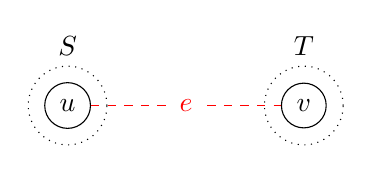
\begin{tikzpicture}
						\node[circle, draw] (u)  at (0,0) {$u$};
						\node[circle, draw] (v)  at (3,0) {$v$};
						\node[circle, draw, dotted, minimum size=1cm, label=$S$] (S) at (0, 0) {};
						\node[circle, draw, dotted, minimum size=1cm, label=$T$] (S) at (3, 0) {};
						\draw[red, dashed] (u) -- (v) node [midway,fill=white] {$e$};
					\end{tikzpicture}
				\end{center}

				\item \textbf{Case 2: } $u$ and $v$ are in the same component $S = (V_S, V_T)$, $u, v \in V_S$:\\
					$G$ is disconnected, hence there is atleast another not empty component $T = (V_T, E_T)$ with $S \neq T$. 
					Considering that $V_T$ is not empty, then there is a vertex $w \in V_T$ such that the edges $e_1 = \{u, w\}$ and $e_2 = \{v, w\}$ exist in $\bar{G}$ (see Case 1). From these considerations, $\bar{G}$ also contains the path $(u, w, v)$ .
				\begin{center}
					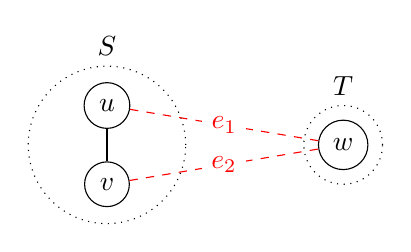
\begin{tikzpicture}
						\node[circle, draw] (u)  at (0,0) {$u$};
						\node[circle, draw] (v)  at (0,-1) {$v$};
						\node[circle, draw] (w)  at (3,-0.5) {$w$};
						\node[circle, draw, dotted, minimum size=2cm, label=$S$] (S) at (0, -0.5) {};
						\node[circle, draw, dotted, minimum size=1cm, label=$T$] (S) at (3, -0.5) {};
						\draw (u) -- (v);
						\draw[red, dashed] (u) -- (w) node [midway,fill=white] {$e_1$};
						\draw[red, dashed] (v) -- (w) node [midway,fill=white] {$e_2$};
					\end{tikzpicture}
				\end{center}
			\end{itemize}

			Therefore, any two vertices in a \emph{disconnected graph} $G$ are connected in $\bar{G}$ either by one or two edges and hereby $\bar{G}$ is connected.\\
		\end{theorem}
	\end{solution} 
	\newpage
	\begin{solution}{4}
		I will prove the theorem that if $u$ and $v$ are the only vertices with odd degree in a graph $G$, then there is a path connecting $u$ and $v$. Our assumption is going to be that there is no path connecting those odd-degree vertices - which we will prove to be a contradiction.
		\begin{theorem}{If $u$ and $v$ are the only vertices of odd degree in a graph then there is a $u$-$v$-path.}
		Let $G = (V, E)$ be a graph with vertices $u,v \in V$ and let $u$ and $v$ be the only vertices with odd degree in G. \\
		Assuming that there is no path connecting $u$ and $v$, then $u$ and $v$ have to be in different components. If they were in the same component, then there had to be a path connecting $u$ and $v$.\\
		Let $A$ be the component of $u$, then $u$ is the only odd-degree vertex in $A$ (as seen above, $v$ is not in $A$). Because $u$ is the only vertex with odd degree in $A$, the sum over the degree of all vertices in $A$ is odd. However, the sum over the degrees over all vertices in a graph has to be even and this leads to the conclusion that $A$ is no valid graph.\\
		This is a contradiction to $A$ being a valid component of $G$, hence the assumption that there is no path connecting $u$ and $v$ must be wrong leaving the only conclusion that there is a $u$-$v$-path.	
		\end{theorem}
	\end{solution}
\end{document}